\section{Evaluation}\label{sec:evaluation}
We have already looked at other results in the literature in Section \ref{sec:practical-results-lit} which gave a decent comparison between some of the algorithms. However, we did not get a lot of knowledge about the datasets, especially the structure of the preference list and distribution of those preferences. Therefore we will conduct an experiment, by benchmarking the implemented algorithms with both real and artificial datasets of varying sizes and preference structures.

\subsection{Research Questions}\label{sec:research-q}
Table \ref{tab:algorithm-comparison} already compared and summarized the algorithms from a theoretical perspective, however some of the results would benefit from further quantification and clarity. For instance, we know that the Popular-CHA algorithm, as described in Section \ref{algo-max-pop}, does not always produce a matching. It would be beneficial to empirically investigate if certain inputs cause this problem. Therefore we will formalize some open questions as research questions, that this experiment hopes to answer:
\begin{enumerate}
    \item What is the effect of different preference distributions on the matchings produced by the different algorithms.
    \item How likely is it for the Popular-CHA algorithm to not produce a matching using different datasets?
    \item How does the Modified-Popular algorithm from Section \ref{impl:mod-max-pop} compare in terms of popularity to the other algorithms.
    \item What is the cost of giving up on strategy proofness in terms of rank, i.e. how well does RSD perform compared to other mechanisms?
    \item Is Popularity a meaningful metric for the student-seminar use case?
    \item What is the impact of short-preference lists on the quality and existence of matchings?
\end{enumerate}

\subsection{Sample Data}
Due to the fact that real data for seminar registrations is mostly kept private, a majority of the benchmark will rely on synthetic data. However, there are a few publicly available datasets available that will be used for evaluation and also for better understanding real-world preference distributions.

\subsubsection{Using graph generators}
Using graph generators to synthetically create instances to the seminar-student matching problem turned out to be a big challenge. Essentially, we would need a graph generator for bipartite, weighted graphs, that also considers the seminar capacity. One option would be generating as many nodes as the total capacity of all seminars, but that could result in duplicate edges or i.e. preferences. Therefore we will use a custom, domain specific mechanism for generating instances.

\subsubsection{Random Uniform Preference Lists}
Probably the simplest way to synthetically generate data, was picking a size for the instance and then generating seminars and students based on a uniform random generator. The preference lists are created by shuffling the list of all seminars for each student. Additionally, we can simply shorten each preference list by a random factor as well for measuring the effect of incomplete-preference lists.

\subsubsection{PrefLib Datasets}
Preflib.org is an open collection of more than 3000 community-contributed datasets of preference data for different domains \cite{PrefLib}. Fortunately, there exist two datasets of students' course preferences at the polish AGU University \cite{preflib-dataset}. The two datasets contain strict and complete preference lists for each students with 9 courses and 146 students or 7 courses and 153 students respectively. Unfortunately there are no capacities given, however those will be computed synthetically using a uniform distribution. An interesting characteristic of those dataset is that in each dataset, all students rank the same seminar with their first preference. I decided to those seminars from the dataset, because I wouldn't assume such a preference distribution in the real world.

\begin{figure}[h!]
    \centering
    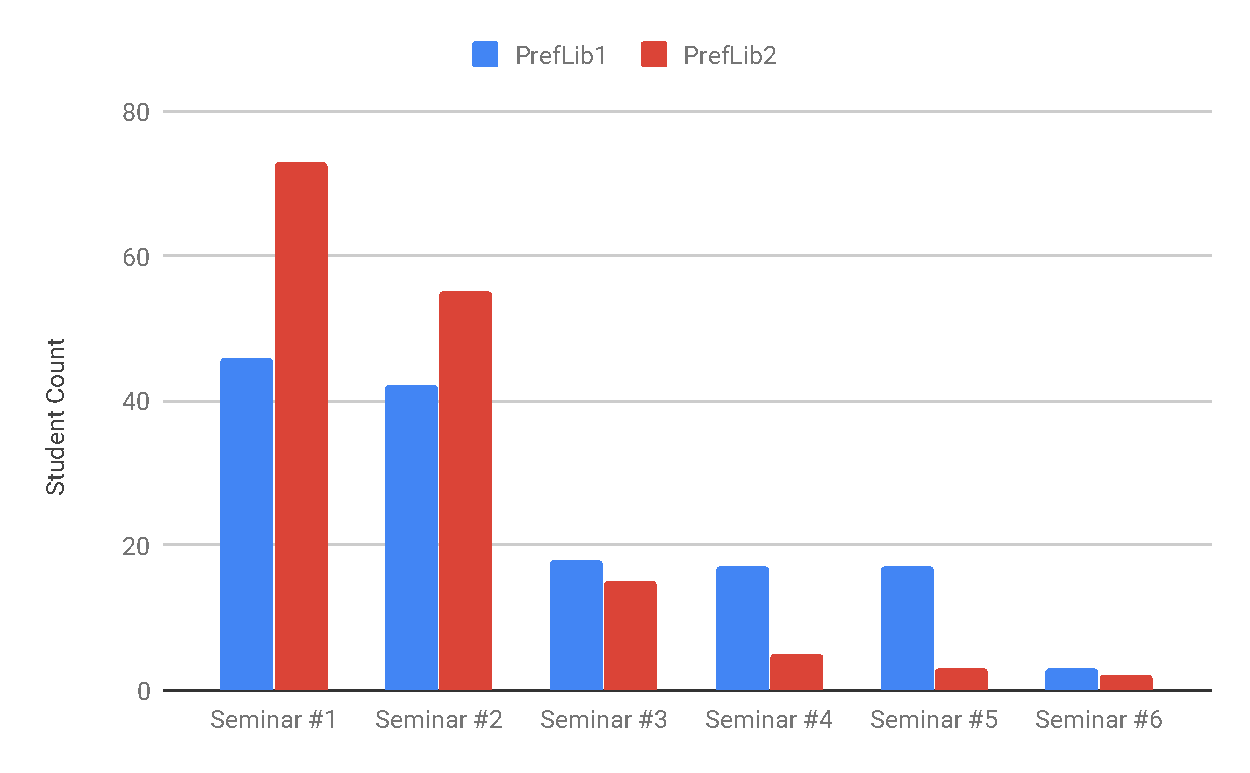
\includegraphics[width=0.8\linewidth]{assets/plots/prelib-distr.pdf}
    \caption{Preference distributions for first-ranked seminars for both PrefLib datasets}
    \label{fig:preflib-distribution}
\end{figure}

Figure \ref{fig:preflib-distribution} shows the preference distributions for the student's first choice in both datasets after removing the always first-ranked seminar. We can see that in both datasets, students clearly strongly prefer two seminars. However in the first dataset, there are 3 more seminars that are also decently popular, while in the second dataset the majority of students really prefers the two dominant seminars. Generally, those datasets indicate that the preference structure is perhaps not likely to be uniformly distributed.

\subsubsection{Random Zipf-Distributed Preference Lists}
To better simulate real-world preference structures than by using a uniform distribution, a power-law distribution can be applied. According to Zipf's law the frequency of a word in a large sample, is proportional to it's position in a frequency table. This law can also be applied for creating synthetic seminar distribution. Using this type of distribution with some additional randomization yields the following preference list structure when seminar and student counts are similar to the first PrefLib dataset:

  \begin{figure}[h!]
    \centering
    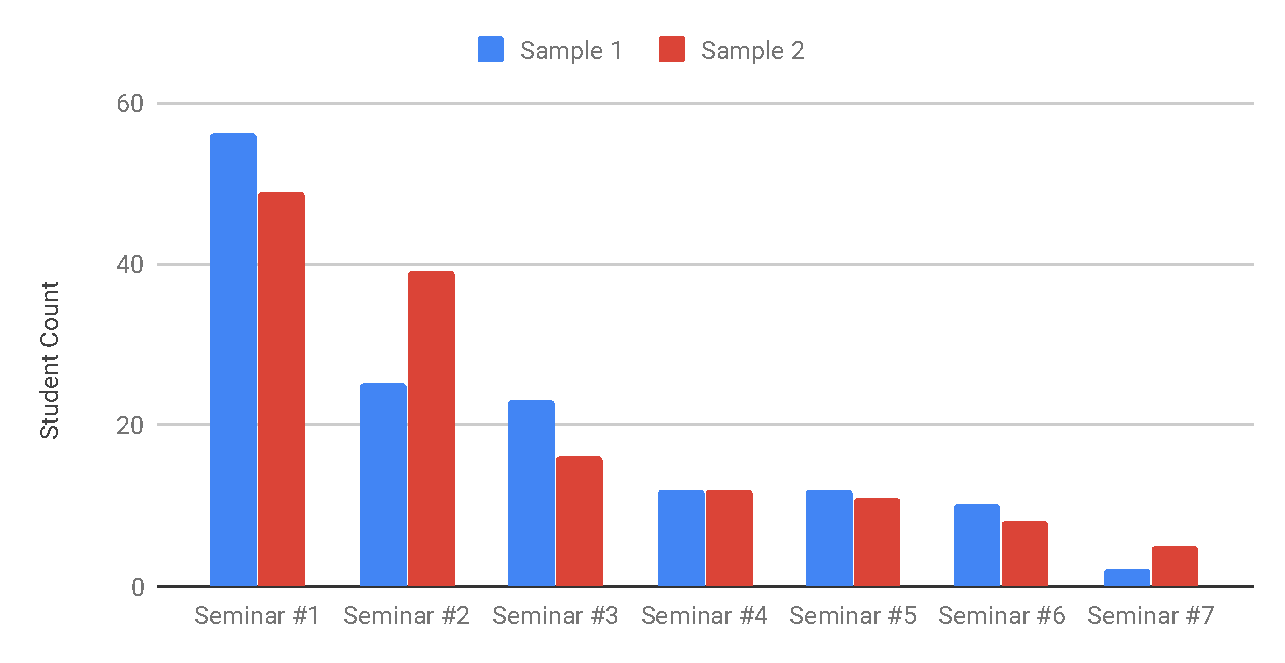
\includegraphics[width=0.8\linewidth]{assets/plots/zipfian-distr.pdf}
    \caption{Two sample Zipfian preference distribution for first-ranked seminars}
    \label{fig:zipfian-distribution}
\end{figure}

To create the dataset, for each student a seminar is randomly drawn using the Zipfian distribution and added to the his preference list until the desired preference-list length has been reached. Comparing Figure \ref{fig:zipfian-distribution} to Figure \ref{fig:preflib-distribution} shows somewhat similar results, which should make this generator relevant for the benchmark. 

\subsection{Methodology}
The goal of this experiment is quantifying some of the optimality criteria defined in Section \ref{sec:optimality} to compare the selection of algorithms empirically and find answers to the research questions proposed in Section \ref{sec:research-q}. Due to the fact that real-world data for student enrollments is not widely available, it is important to note that the results of this experiment will be biased by the selection of data available. However, by using the available real datasets and a few different synthetic datasets it should be possible to find answers to the proposed research questions and to better understand the differences of different approaches.

\subsubsection{Benchmark Setup}
The benchmark is performed by a Kotlin program that generates test data and then executes each of the algorithms with the same input. The program then collects the results and computes statistics on each matching, which are saved into a file. When using synthetic data, the program will generate between 10-50 different instances to account for the randomness. The following types of instances will be used:
\begin{enumerate}
  \item PrefLib Datasets
  \item Medium Sized Random Dataset ($\sim$100 students)
  \begin{enumerate}
    \item with uniform preference distribution
    \item with Zipfian preference distribution
  \end{enumerate}
  \item Large Sized Random Dataset ($\sim$1000 students)
  \begin{enumerate}
    \item with uniform preference distribution
    \item with Zipfian preference distribution
  \end{enumerate}
\end{enumerate}

\subsubsection{Metrics}
We already know that all of the algorithms under considerations produce pareto-optimal matchings, however it will be necessary to measure popularity. If the Popular-CHA algorithm finds a matching, we know that it's the popular matching, however if the algorithm cannot find a matching it could be possible that one of the other algorithms produces such a matching. In general, given the definitions for Popularity that we have used before, it is not possible to check if a given matching is popular without comparing it to all other matchings. However this is infeasable due to the exponential runtime complexity of that comparison, which is why we will just compare the matchings produced by the five algorithms for Popularity. Given two matchings $m, m' \in \mathcal{M}$, we say that $m$ is more popular than $m'$ if the number of students prefering $m$ is greater than the number of students prefering $m'$. 
In addition to comparing Popularity, the following other metrics will be used:
\begin{itemize}
  \item \textbf{Profile}: The profile of the matching as defined in Section \ref{sec:profile} given as an array.
  \item \textbf{Average Rank \& Standard Deviation}: The average and standard deviation of the matched students' ranks. A matched student's rank corresponds to the position of his match on his preference list. In case there are unassigned students, two numbers will be given for this metric. First the metric excluding unassigned students is given and then in parentheses the metrics including unassigned students, weighted with the maximum rank is given.
  \item \textbf{Worst Rank}: In conjunction with the previous metric, we will also look at the worst rank that exists in a matching.
  \item \textbf{Unassigned-Count}: The number of unassigned students in a matching.
  \item \textbf{Runtime}: The runtime of the algorithm in milliseconds. Only the runtime of the actual algorithm in C++ is measured without parsing the input data or printing the result.
  \item \textbf{Existence}: This metric is only interesting for the Popular-CHA algorithm and will indicate if the algorithm was able to compute a matching for a given instance.
\end{itemize}

These metrics should be a sufficient selection to quantify a matching's optimality and therefore should make it possible to answer the research questions from section \ref{sec:research-q}.

\subsection{Results}

\subsubsection{PrefLib1 dataset}
The PrefLib datasets contain strict, complete preferences for a small number of students and seminars. Table \ref{tab:results-preflib1} shows results for executing the algorithms on the first dataset. Unfortunately, the Popular CHA algorithm did not compute a matching, however we can also see that the Mod-Popular algorithm computed a matching that ties in popularity with the matching produced by the Hungarian algorithm. Unsurprisingly, in terms of rank the Hungarian algorithm produces the best matching with an average rank of 1.513 and a standard deviation of 0.829.

\begin{table}[h!]
  \centering
  \resizebox{\textwidth}{!}{%
  \begin{tabular}{|l|l|l|l|l|l|}
  \hline
  Metric & RSD & Max PaCHA & Hungarian & Popular CHA & Mod-Popular \\ \hline
  Average Rank & 1.787 & 1.924 & \cellcolor[HTML]{9AFF99}1.513 & \cellcolor[HTML]{FFCCC9}n/a & 1.276 (2.342) \\ \hline
  Rank SD & 1.136 & 1.426 & \cellcolor[HTML]{9AFF99}0.829 & \cellcolor[HTML]{FFCCC9}n/a & 0.540 (3.079) \\ \hline
  Unassigned-Count & 0 & 0 & 0 & \cellcolor[HTML]{FFCCC9}146 & \cellcolor[HTML]{FFCCC9}16 \\ \hline
  Runtime & <1ms & 19ms & 13ms & 1ms & 1ms \\ \hline
  More Popular & 1.5 & 1.5 & \cellcolor[HTML]{9AFF99}3.5 & 0 & \cellcolor[HTML]{9AFF99}3.5 \\ \hline
  Worst Rank & 7 & 7 & 4 & - & 3 / Unassigned \\ \hline
  Exists & yes & yes & yes & \cellcolor[HTML]{FFCCC9}no & yes \\ \hline
  \end{tabular}%
  }
  \caption{Summary of the results for PrefLib1}
  \label{tab:results-preflib1}
\end{table}

When not taking the unassigned students into account, the Mod-Popular CHA algorithm performs even better on the rank metrics, however if taking the unassigned students into account it performs worst among all algorithms. Figure \ref{fig:preflib1-rank-distribution} shows the rank distribution for the algorithms that produced a matching and makes clear that, the Mod-Popular CHA algorithm assigns more students to their first rank at the cost of leaving a lot of students unassigned. 

\begin{figure}[h!]
  \centering
    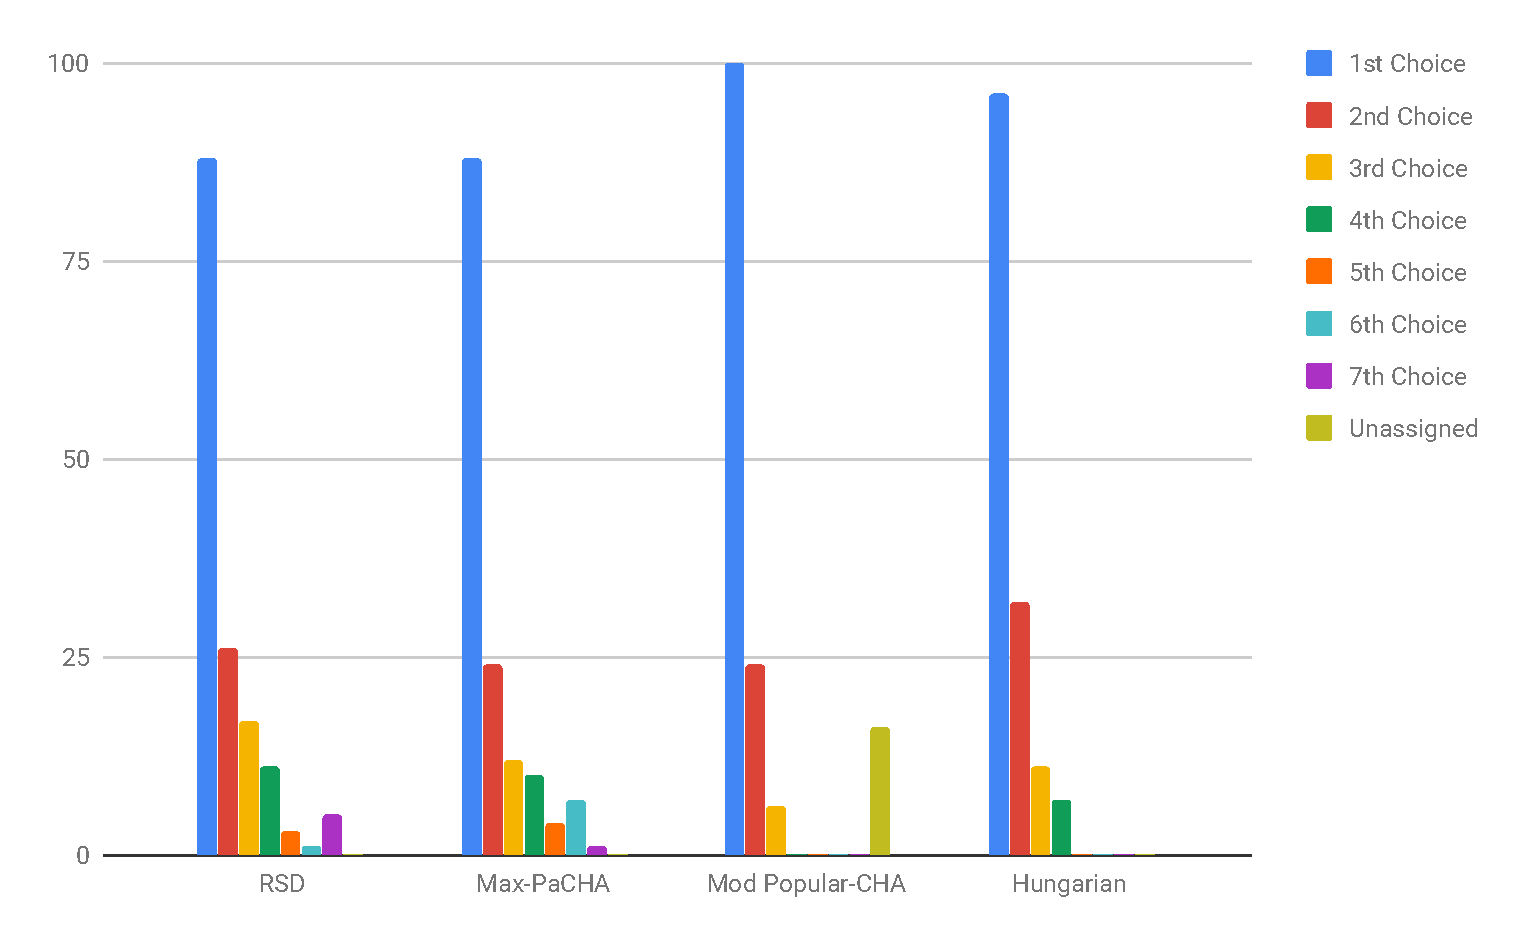
\includegraphics[width=0.9\linewidth]{assets/plots/preflib1-ranks.pdf}    
    \caption{Rank distribution for PrefLib1 Dataset. Note: Popular CHA failed.}
    \label{fig:preflib1-rank-distribution}
\end{figure}

What else is surprising with this instance is that the greedy RSD algorithm performs better than Max PaCHA in regards to the rank metric, even though both are of maximum cardinality. Surprisingly the algorithms also tie for popularity for this instance, even though the RSD performs better from a rank perspective. Runtime wise, there are no surprises other than the fact that the Hungarian algorithm is faster than Max PaCHA for this instance. However, with this size of input the runtime results are not that significant.

\subsubsection{PrefLib2 dataset}
\begin{table}[h!]
  \centering
  \resizebox{\textwidth}{!}{%
  \begin{tabular}{|l|l|l|l|l|l|}
  \hline
  Metric & RSD & Max PaCHA & Hungarian & Popular CHA & Mod-Popular \\ \hline
  Average Rank & 1.712 & \cellcolor[HTML]{FFCCC9}1.758 & \cellcolor[HTML]{9AFF99}1.640 & 1.686 & 1.686 \\ \hline
  Rank SD & 0.797 & \cellcolor[HTML]{FFCCC9}0.878 & \cellcolor[HTML]{9AFF99}0.728 & 0.787 & 0.787 \\ \hline
  Unassigned-Count & 0 & 0 & 0 & 0 & 0 \\ \hline
  Runtime & <1ms & 41ms & 45ms & 9ms & 10ms \\ \hline
  More Popular & 1 & 0 & \cellcolor[HTML]{96FFFB}2 (+2 Ties) & \cellcolor[HTML]{96FFFB}2 (+2 Ties) & \cellcolor[HTML]{96FFFB}2 (+2 Ties) \\ \hline
  Worst Rank & 5 & 5 & 3 & 3 & 3 \\ \hline
  Exists & yes & yes & yes & yes & yes \\ \hline
  \end{tabular}%
  }
  \caption{Summary of the results for PrefLib2}
  \label{tab:results-preflib2}
\end{table}

Table \ref{tab:results-preflib2} shows the results for the PrefLib2 dataset. We can see that the Popular CHA algorithm finds a matching, which is why the last two columns are identical. What's interesting about the results is that the the matchings produced by the Hungarian and Popular CHA algorithm tie in popularity, even though they are different in regards to the rank metrics. 

What else stands out is that RSD again produces a better matching than Max PaCHA in regards to the rank metrics. In fact, the matching produced by the Max PaCHA algorithm performs worst in terms of rank, even though its runtime is the second highest. Overall the runtimes are still low, with all of them being lower than 50ms, which should make all algorithms usable for real world applications for similarly sized instances. However it has to be noted that the matching produced by RSD gets close in terms of rank to the matching produced by the Hungarian algorithm, even though the it is about 50 times faster.

\begin{figure}[h!]
  \centering
    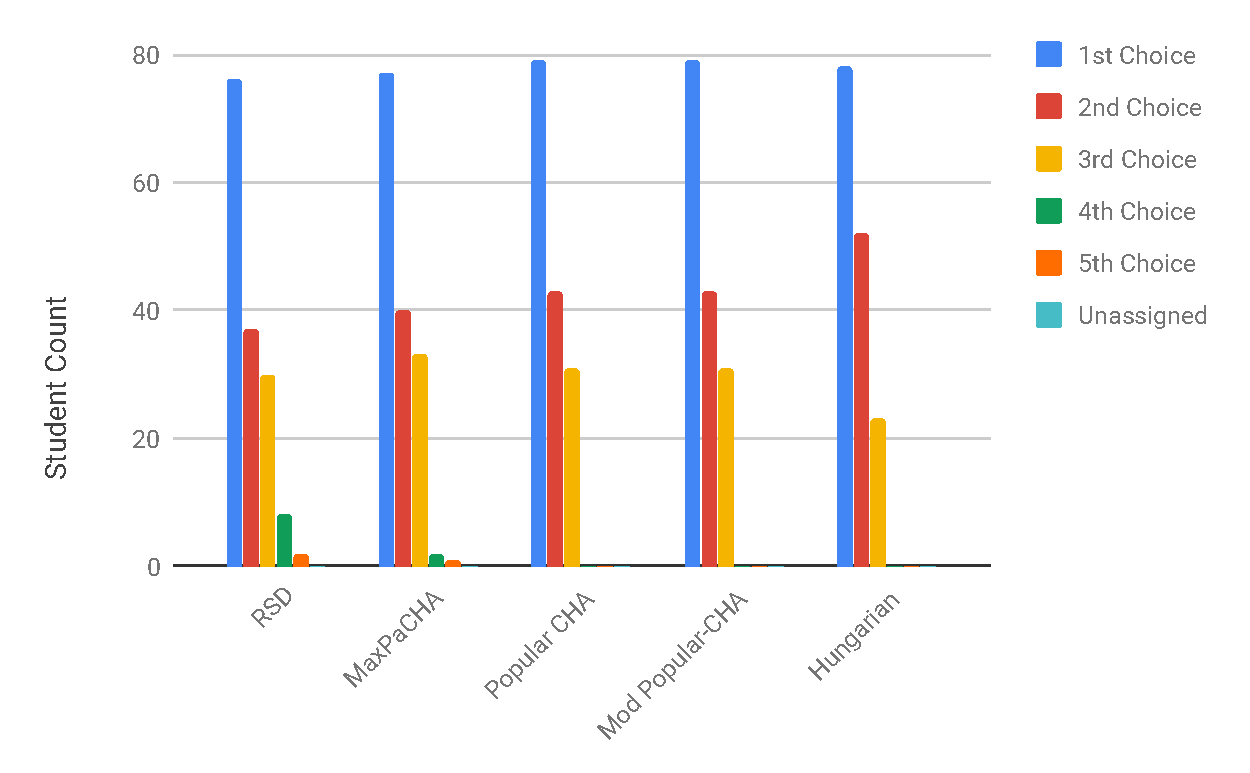
\includegraphics[width=0.9\linewidth]{assets/plots/preflib2-ranks.pdf}    
    \caption{Rank distribution for PrefLib2 Dataset.}
    \label{fig:preflib2-rank-distribution}
\end{figure}

Figure \ref{fig:preflib2-rank-distribution} shows the preference distribution of all five algorithms. We can see that RSD and Max-PaCHA assign some students to their 4th or 5th choice, which explains why they perform worse in terms of rank. Unsurprisingly the matching produced by the Hungarian algorithm has the best rank-profile.

\subsubsection{Small Zipfian datasets}

\begin{table}[h!]
  \centering
  \resizebox{\textwidth}{!}{%
  \begin{tabular}{|l|l|l|l|l|l|}
  \hline
  Metric & RSD & Max PaCHA & Hungarian & Popular CHA & Mod-Popular \\ \hline
  Average Rank & 1.893 (2.014) & 1.910 & \cellcolor[HTML]{9AFF99}1.481 & 1.646 & 1.523 (1.913) \\ \hline
  Rank SD & 1.451 (1.782) & 1.457 & \cellcolor[HTML]{9AFF99}0.716 & 1.034 & 0.874 (2.121) \\ \hline
  Unassigned-Count & 2 & 0 & 0 & 0 & \cellcolor[HTML]{FFCCC9}7 \\ \hline
  Runtime & \textless{}1ms & 54ms & 60ms & 7ms & 10ms \\ \hline
  More Popular & 1 & 1.65 & 3.05 & 0.7 & \cellcolor[HTML]{9AFF99}3.6 \\ \hline
  Worst Rank & \cellcolor[HTML]{FFCCC9}8 & \cellcolor[HTML]{FFCCC9}8 & \cellcolor[HTML]{9AFF99}5 & \cellcolor[HTML]{9AFF99}5 & 6 \\ \hline
  Exists & yes & yes & yes & \cellcolor[HTML]{FFCCC9}4/50 exist & yes \\ \hline
  \end{tabular}%
  }
  \caption{Average results for small Zipfian dataset with 50 runs}
  \label{tab:results-zipfian-small}
\end{table}

Since the Zipfian datasets have a somewhat similar preference distribution as the PrefLib datasets we should see similar results, however parameters can be tuned such as preference list length and student count. We will begin by looking at a similarly sized dataset as the Preflib datasets and then begin deviating the preference list length and finally student \& seminar count. Table \ref{tab:results-zipfian-small}
shows the average results for 50 test runs using the Zipfian Dataset with 10 seminars and about 200 students. Out of the 50 instances, the Popular CHA algorithm only found a matching for four instances. When it found a matching, it did so quite fast and the matching was on average better rank-wise than all other algorithms except for the Hungarian algorithm. In terms of popularity, the Mod-Popular CHA algorithm actually outperformed all algorithms (equal to Popular-CHA if the matching exists) for most instances, even though rank-wise it does not perform as well as the Hungarian algorithm. However, the Hungarian algorithm produced more popular matchings than most other algorithms, and for some instances even more popular than the Mod-Popular CHA algorithm.

\subsubsection{Large Zipfian datasets}
Using a large dataset with a Zipfian distribution yields similar results. Table \ref{tab:results-zipfian-medium} summarizes the average results for 10 test runs with datasets that contain about 2500 students and 35 seminars.

\begin{table}[h!]
  \centering
  \resizebox{\textwidth}{!}{%
  \begin{tabular}{|l|l|l|l|l|l|}
  \hline
  Metric & RSD & Max PaCHA & Hungarian & Popular CHA & Mod-Popular \\ \hline
  Average Rank & 1.911 (5.287) & \cellcolor[HTML]{FFCCC9}2.109 & \cellcolor[HTML]{9AFF99}1.824 & - & 1.694 (4.746) \\ \hline
  Rank SD & 1.225 (10.41) & \cellcolor[HTML]{FFCCC9}1.383 & \cellcolor[HTML]{9AFF99}1.029 & - & 1.087 (9.967) \\ \hline
  Unassigned & \cellcolor[HTML]{FFCCC9}10\% & \cellcolor[HTML]{9AFF99}0\% & \cellcolor[HTML]{9AFF99}0\% & 100\% & \cellcolor[HTML]{FFCCC9}8.6\% \\ \hline
  Runtime & \cellcolor[HTML]{9AFF99}3ms & 2190ms & \cellcolor[HTML]{FFCCC9}65730ms & - & \cellcolor[HTML]{9AFF99}168ms \\ \hline
  More Popular & 1.1 & 1.65 & 3 & 0 & \cellcolor[HTML]{9AFF99}4 \\ \hline
  Worst Rank & 7 & 7 & \cellcolor[HTML]{9AFF99}6 & - & 7 \\ \hline
  Exists & yes & yes & yes & \cellcolor[HTML]{FFCCC9}0/10 & yes \\ \hline
  \end{tabular}%
  }
  \caption{Average results for large Zipfian dataset (2500 Students) with 10 runs}
  \label{tab:results-zipfian-medium}
\end{table}

Again, the Popular CHA algorithm was not very successful and found no matching in any of the test runs. However, the Mod-Popular CHA algorithm always produced more popular matchings than all of the other algorithms, even though 8.6\% of the students were left unassigned on average. When taking the unassigned students out of the rank metrics, the Mod-Popular CHA algorithm produces matchings with the best average rank and standard deviation, while having the second lowest runtime. In contrast to that, the Hungarian algorithm always assigned all students, however needed on average 65 seconds to do so. This confirms the theoretical observations about runtime and shows that using the Hungarian algorithm is potentially not feasible for large instances.

\begin{figure}[h!]
  \centering
    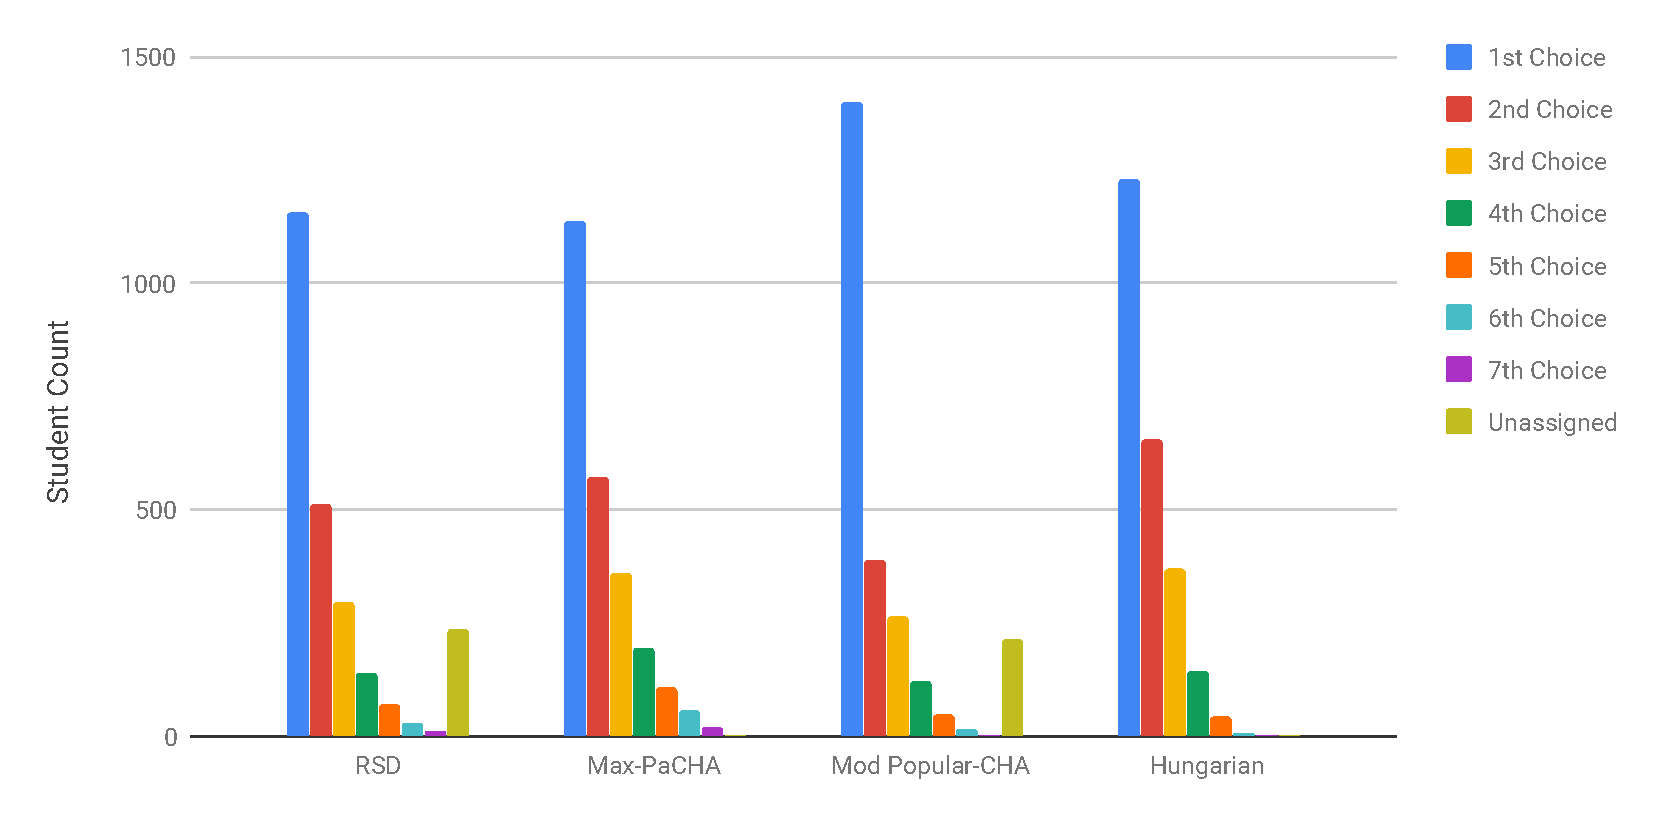
\includegraphics[width=0.9\linewidth]{assets/plots/zipfian-medium.pdf}
    \caption{Rank distribution for large Zipfian dataset.}
    \label{fig:zipfian-medium-distribution}
\end{figure}

Figure \ref{fig:zipfian-medium-distribution} shows the rank distributions for all algorithms but Popular CHA. We can see that Mod Popular-CHA is able to outperform the other algorithms in terms of popularity by maximizing the number of students being assigned to their first choice. However, the Hungarian algorithm produced more balanced matchings, where the most students were assigned to their top three choices, while also leaving no student unassigned.

\subsubsection{Large uniform dataset with incomplete preferences}
This large uniform dataset contains 50 seminars and 5000 students, who each randomly picked 10 seminars with equal probability.  

\begin{table}[h!]
  \centering
  \resizebox{\textwidth}{!}{%
  \begin{tabular}{|l|l|l|l|l|l|}
  \hline
  Metric & RSD & Max PaCHA & Hungarian & Popular CHA & Mod-Popular \\ \hline
  Average Rank & 1.119 (1.265) & \cellcolor[HTML]{FFCCC9}1.133 & \cellcolor[HTML]{9AFF99}1.041 & 1.093 & 1.083 \\ \hline
  Rank SD & 0.647 (2.778) & \cellcolor[HTML]{FFCCC9}0.713 & \cellcolor[HTML]{9AFF99}0.2 & 0.508 & 0.486 \\ \hline
  Unassigned & 0.28\% & 0\% & 0\% & 0\% (90\%) & 0\% \\ \hline
  Runtime & 13ms & 6175ms & \cellcolor[HTML]{FFCCC9}55815ms & 257ms & 221ms \\ \hline
  More Popular & 1.65 & 1.15 & \cellcolor[HTML]{9AFF99}3.45 & 0.3 & \cellcolor[HTML]{9AFF99}3.45 \\ \hline
  Worst Rank & 10 & 10 & \cellcolor[HTML]{9AFF99}2 & 8 & 10 \\ \hline
  Exists & yes & yes & yes & 1/10 & yes \\ \hline
  \end{tabular}%
  }
  \caption{Average results for large uniform dataset with incomplete preferences.}
  \label{tab:results-uniform-large}
\end{table}

Table \ref{tab:results-uniform-large} shows the average results when executing each algorithm 10 times. Unfortunately the Popular CHA algorithm only found a matching for one out of the 10 instances, but when it did it performed quite well in terms of rank. However, the Mod-Popular CHA algorithm was on average able to find better matchings in less time than the Popular CHA mechanism. What also stands out is that Mod-Popular CHA and the Hungarian algorithm are tied for popularity in every instance, but runtime wise Mod-Popular CHA performs far better than the Hungarian algorithm. What needs to be noted though, is that the Hunarian algorithm outperforms all other algorithms in terms of profile by having the worst rank in all matchings be 2. All algorithms assign more than 94\% of the students to their first choice, but the Hungarian algorithm only assigns students to their first or second choice.  

\subsubsection{Large uniform dataset with complete preferences}
When using the same size dataset as before, but with complete preference lists, the results show some interesting insights. Table \ref{tab:results-uniform-large-complete} shows that Popular-CHA found a matching for every instance, which helps answer the question if preference list length has an effect on Popular CHA. For this dataset, Popular CHA and the Hungarian algorithm always produce matchings of the same popularity, which means that there exists more than one popular matching for every instance. 

\begin{table}[h!]
  \centering
  \resizebox{\textwidth}{!}{%
  \begin{tabular}{|l|l|l|l|l|l|}
  \hline
  Metric & RSD & Max PaCHA & Hungarian & Popular CHA & Mod-Popular \\ \hline
  Average Rank & \cellcolor[HTML]{FFCCC9}1.198 & 1.190 & \cellcolor[HTML]{9AFF99}1.039 & \cellcolor[HTML]{9AFF99}1.076 & \cellcolor[HTML]{9AFF99}1.076 \\ \hline
  Rank SD & \cellcolor[HTML]{FFCCC9}1.543 & 1.469 & \cellcolor[HTML]{9AFF99}0.193 & \cellcolor[HTML]{9AFF99}0.453 & \cellcolor[HTML]{9AFF99}0.453 \\ \hline
  Unassigned & 0\% & 0\% & 0\% & 0\% & 0\% \\ \hline
  Runtime & 11ms & 7922ms & \cellcolor[HTML]{FFCCC9}57141ms & 228ms & 219ms \\ \hline
  More Popular & 0.5 & 0.5 & \cellcolor[HTML]{9AFF99}3 & \cellcolor[HTML]{9AFF99}3 & \cellcolor[HTML]{9AFF99}3 \\ \hline
  Worst Rank & \cellcolor[HTML]{FFCCC9}30 & \cellcolor[HTML]{FFCCC9}27 & \cellcolor[HTML]{9AFF99}2 & 9 & 9 \\ \hline
  Exists & yes & yes & yes & \cellcolor[HTML]{9AFF99}10/10 & yes \\ \hline
  \end{tabular}%
  }
  \caption{Average results for large uniform dataset with complete preferences.}
  \label{tab:results-uniform-large-complete}
\end{table}

Another things that stands out is the fact that RSD and Max PaCHA produce matchings with high worst-ranks of 30 and 27 respectively. Overall these two algorithms perform worse or equal on all metrics than Popular CHA and the Hungarian algorithm, which makes them less appealing for this kind of dataset. Given the low average runtime of 219ms the Mod-Popular CHA algorithm seems to be a good option when the size of the instance is too large for the Hungarian, while still performing well on the rank-related metrics. Even though Popular-CHA and the Hungarian algorithm tie in popularity, it should be assumed that a matching with a worst rank of 2 is more popular among the students than a matching of worst rank 9. 

\subsection{Conclusion}
The experiments have revealed some interesting insights that should help answering the research questions from section \ref{sec:research-q}.

\begin{enumerate}
  \item \textbf{Effect of different preference distributions:} Unsurprisingly, the algorithms performed better on the rank metrics, when the preferences were distributed uniformly. In fact, the Hungarian algorithm was able to assign on average more than 94\% (table \ref{tab:results-uniform-large-complete}) of the students to their first choice when the preference distribution was uniform.
  \item \textbf{Failure rate of Popular-CHA:} The experiments have shown that Popular-CHA fails to find a matching quite often, especially if the preference lists are short and not uniformly distributed. When using the Zipfian datasets (tables \ref{tab:results-zipfian-medium}, \ref{tab:results-zipfian-small}), Popular-CHA only found a matching for 4/60 instances. Even for uniform distributions and incomplete preference lists (table \ref{tab:results-uniform-large}) the algorithm only found a matching for 1/10 instances. Making the preference lists complete makes it easier for the algorithm to find matchings as shown in table \ref{tab:results-uniform-large-complete}.
  \item \textbf{Performance of Mod-Popular-CHA:} The modified version of Popular-CHA was able to find comparatively good matchings in a short amount of time, while also usually producing more or equally popular, matchings as the other algorithms. For many instances Mod-Popular-CHA tied the Hungarian algorithm for popularity and was able to produce good matchings in terms of the rank metrics in a fraction of the time.
  \item \textbf{Cost of giving up on strategy-proofness:} Surprisingly RSD produced on average better matchings on most metrics than Max-PaCHA, while also being by far the fastest algorithm. However, RSD usually produced the highest percentage of unassigned students, but the modified Popular-CHA algorithm usually outperformed RSD on most metrics, while also having a relatively low runtime. In the real-world datasets (PrefLib), RSD left no students unassigned and got close to the Hungarian algorithm in terms of rank, but also had 7 as the worst rank, compared to 4 for the Hungarian algorithm. 
  \item \textbf{Popularity as a meaningful metric:} For many instances we could not find the one popular matching, as it simply did not exist, but when it did, the worst rank, average rank and rank standard deviation was higher than what the Hungarian algorithm produced. Another interesting insight was that matchings produced by Mod-Popular-CHA usually tied in popularity with those produced by the Hungarian algorithm, even though Mod-Popular-CHA often left a few students unassigned. For instance in Figure \ref{fig:zipfian-medium-distribution}, Mod-Popular-CHA left on average 8.6\% of the students unassigned but the matchings were still classified as more popular than the matchings produced by the Hungarian algorithm. This shows that a popular matching can maximize the number of students ranked to their first choice at the cost of some students being matched to a low-ranking seminar or even none. This makes it questionable, whether popularity is meaningful for the student and seminar usecase, as it should be a goal to assign as many students as possible and to make all students equally satisfied with their match instead of finding the biggest possible subset of students, where everyone is satisfied.
  \item \textbf{The effect of short preference lists:} The experiments have shown that short preference lists make it more likely for Popular-CHA to not find a matching, as well as making it more likely for RSD to produce matchings with more unassigned students.
\end{enumerate}

In summary, the matchings produced by the Hungarian algorithm usually perform best in all of the metrics, except for runtime where it performs the worst by far. However, for the student-seminar use case that should not be a problem, because most instances will be smaller than what we have tested with. In fact, when using the real world datasets (see Table \ref{tab:results-preflib1} and \ref{tab:results-preflib2}), the runtime differences for the different mechanisms were insignifcant. For large instances, the modified Popular-CHA algorithm performed well and it could still be optimized even further for matching more students. The algorithm as it was in described in section \ref{impl:mod-max-pop}, does not try to assign students that were left unmatched by the Hopcroft-Karp algorithm, which could easily be done by either using a simple mechanism like RSD or even using the Hungarian algorithm on the set of unassigned students. Neither modification guarantees that the final matching would be popular or of maximum cardinality, but it could improve the matching. Therefore it would make the Mod-Popular-CHA algorithm a fast heuristic that should, according to the experiments, perform better than RSD and Max-PaCHA for most instances, while still keeping the runtime low.